\subsection{VRP of 50-Delta Options}

The volatility risk premium is expressed as a simple ratio of the implied volatility priced into the options contract and the realized volatility computed from the methodology mentioned above. 
$$ VRP = IV / RV $$
The following violin plot shows the distribution of the volatility of the volatility risk premium across different tickers and asset classes.

\begin{figure}[H]
    \centering
    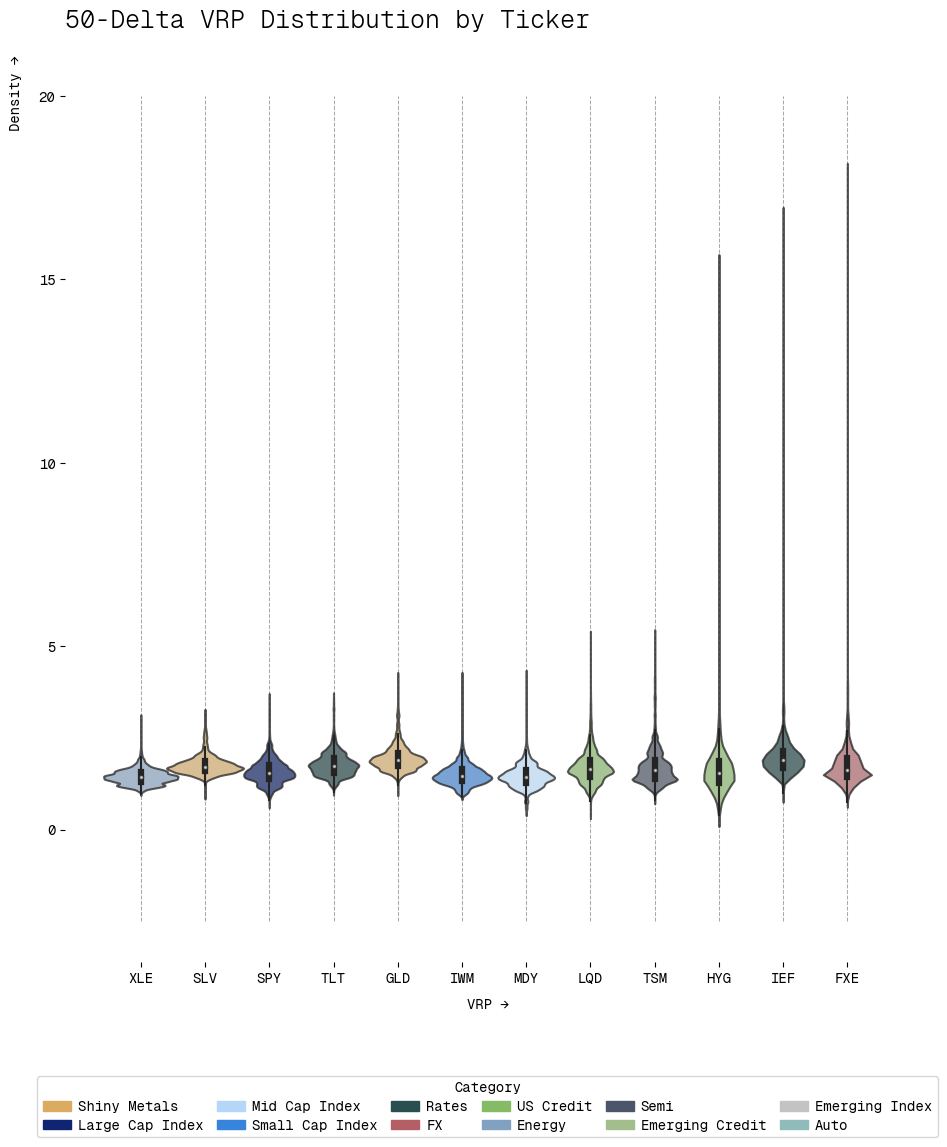
\includegraphics[width=1\textwidth]{images/atm_vrp_violin.png}
    \caption{Distribution of Volatility Risk Premium}
    \label{fig:atm_vrp_violin}
\end{figure}


There are few interesting and apparent insights:
\begin{enumerate}
    \item The ticker which have visibly very long tails are the tickers that are directly affected by interest rates, for example, currency values,  Treasury bond ETFs and credit ETFs.  In the preceding section where we modelled the realized volatility, we have already shown that the interest rate dependent tickers show the slowest mean reversion or a high persistence of volatility. This makes intuitive sense because a lingering volatility would also keep the volatility risk premium high as mean reversion is slow. This could also very well be a data artefact. The last five years which is also the time period of the sample, have seen many interest rate regimes and the market has been pricing in a lot of uncertainty.  These long tails in interest rate dependent tickers appear likely to happen around FOMC meetings. It is interesting to note that the the 20 year treasury bond ETF (TLT) is an exception to this phenomenon probably due to its long term nature.
    \item The volatility risk premium also show a richer variation among different asset classes. This is apparent when we look at the univariate distributions for few tickers. Here, the Gold commands the highest volatility risk premium as the distribution looks significantly to the right that is followed by 20 year Treasury bonds. The VRP of the Energy ETF (XLE) has the lowest variability while the VRP of the Large Cap Index (SPY) has the highest variability. 
\end{enumerate}

\begin{figure}[H]
    \centering
    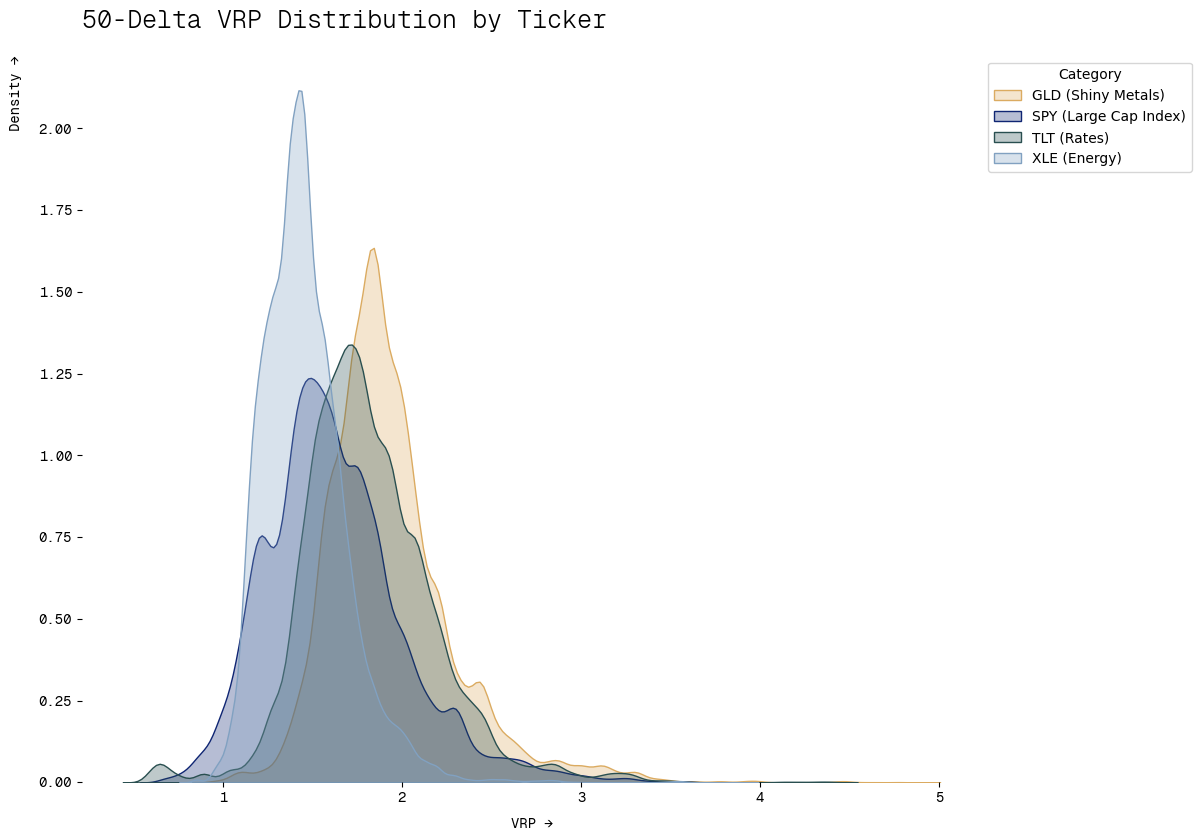
\includegraphics[width=1\textwidth]{images/kde_vrp_atm.png}
    \caption{Distribution of Volatility Risk Premium}
    \label{fig:kde_vrp_violin}
\end{figure}


When we look at the VRP of the OTM options, they are dominated by extremely heavy tails, the length of tails again look highly correlated with interest-rate dependence.

\subsection{VRP of 25 to 30-Delta Options}

When we look at the VRP of the OTM options, they are dominated by extremely heavy tails, the length of tails again look highly correlated with interest-rate dependence.

\begin{figure}[H]
    \centering
    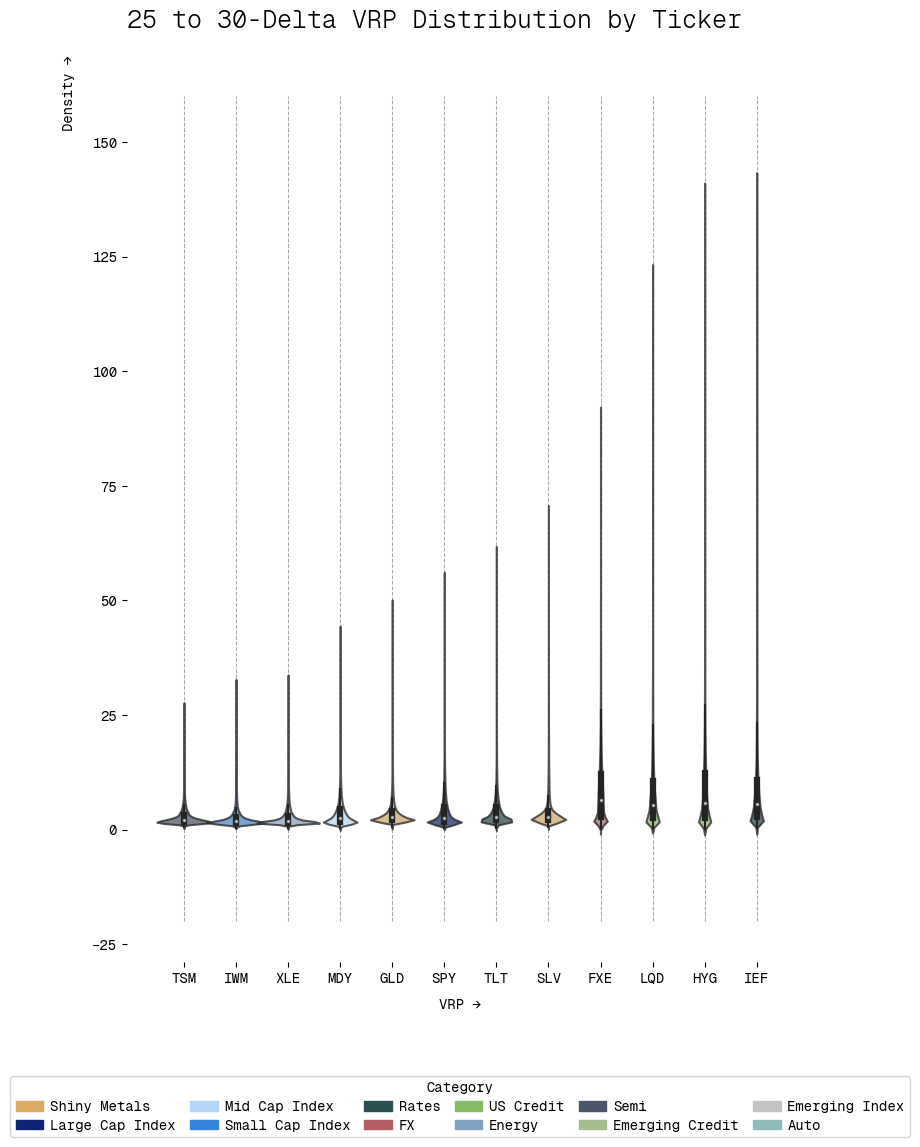
\includegraphics[width=1\textwidth]{images/otm_vrp_violin.png}
    \caption{Distribution of Volatility Risk Premium}
    \label{fig:otm_vrp_violin}
\end{figure}